\documentclass[11pt]{scrartcl}

\usepackage{ucs}
\usepackage[utf8x]{inputenc}
\usepackage[T1]{fontenc}
\usepackage[ngerman]{babel}
\usepackage{amsmath,amssymb,amstext}
\usepackage{graphicx}
\usepackage[justification=RaggedRight, singlelinecheck=false]{caption}


\title{Fortgeschrittenen Praktikum Teil 1: IKF}
\subtitle{Versuch 1: $\gamma \gamma$ - Koinzidenzen \\ Betreuer: Alexander Schottelius}

\author{Gruppe 1: Reinhold Kaiser, Florian Stoll}

\date{14.04.2018}

\begin{document}
\maketitle
\newpage
\tableofcontents
\newpage

\section{Zielsetzung}
In dem Versuch $\gamma$-$\gamma$-Koinzidenzen sollen für zwei Beispiele die Winkelverteilung zweier gleichzeitig entstehender Photonen
gemessen werden. Zum Einen entsteht beim Betazerfall von $^{22}Na$ ein Positron, welches wiederum mit
einem Elektron zu zwei $\gamma$-Quanten annihiliert. Zum Anderen zerfällt $^{60}Co$ zu $^{60}Ni$
und dieses dann über Kaskaden in den Grundzustand. Dabei werden zwei $\gamma$-Quanten emittiert,
deren Winkelkorrelation gemessen werden soll. Physikalisch relevant sind die Messungen von 
Winkelverteilungen, weil durch sie auf die Spin- und Drehimpulsquantenzahlen der angeregten Zustände 
geschlossen werden kann.


\section{Theoretische Grundlagen}

\subsection{Wechselwirkungen elektromagnetischer Strahlung mit Materie}

Um $\gamma$-Strahlung nachweisen zu können macht man sich die Beobachtung der drei Wechselwirkungsprozesse von $\gamma$-Strahlung mit Materie zu Nutze. Diese Wechselwirkungsprozesse liefern, je nach Energiebereich und Detektormaterial, einen unterschiedlichen Beitrag zum gesamten Spektrum. Der Photoeffekt dominiert bei Photonenenergien im keV-Bereich, wohingegen der Compton-Effekt überwiegend im Bereich von 100 keV bis wenige MeV relevant ist. Der Paarbildungsprozess dominiert dagegen bei Energien im MeV-Bereich.

\paragraph{Der Photo-Effekt}

Beim Photoeffekt wird ein Photon von einem Hüllenelektron absorbiert. Es kommt zum vollständigen Energieübertrag an das Elektron, wodurch es aus seiner Bindung mit dem Atomkern gelöst wird und das Atom verlässt. Damit dieser Vorgang stattfinden kann, muss die Energie $E_\gamma$ des einfallenden Photons größer sein als die Bindungsenergie $E_b$ des Elektrons. Je nachdem, in welcher Elektronenschale sich das Elektron befindet, variiert diese Bindungsenergie. Wegen der Impulserhaltung werden bevorzugt Elektronen aus den beiden innersten Schalen herausgelöst. Die kinetische Energie des emitierten Eletrkons folgt dabei der Beziehung

\begin{align}
E_{kin}=E_\gamma - E_b
\end{align}

Da nun in einer der energetisch niedrigeren Schalen ein Elektron fehlt, tritt an dessen Stelle ein Elektron aus einem energetisch höheren Niveau. Die dabei freiwerdende Energie wird in Form eines charakteristischen Photons abgestrahlt. Begünstigt wird der Photoeffekt durch eine Ordnungszahl des Targetatoms und niedrige Photonenenergien.

\paragraph{Der Compton-Effekt}

Trifft ein Photon auf ein schwach gebundenes Elektron eines Atoms, so wird durch einen elastischen Stoß ein Teil seines Impulses und seiner Energie auf dieses Elektron übertragen. Das Elektron verlässt das Atom, während das gestreute Photon an Energie verliert. Der Energieverlust des gestreuten Photons führt zu einer Frequenzänderung. Je nach Streuwinkel verändert sich dieser Energieübertrag an das Photon. Bei einer Streuung um $180^\circ$ wird der Übertrag maximal. Der Wirkungsquerschnitt steigt dabei mit zunehmender Kernladungszahl und nimmt mit steigender Photonenenergie ab. 

\subsection{Die Paarvernichtung}
Wie jedes Elementarteilchen besitzt auch das Elektron ein Anti-Teilchen mit gleichem Spin und gleicher Ruhemasse, jedoch mit entgegengesetzter Ladung. Dieses wird als Positron bezeichnet. Als Formelzeichen verwendet man hier $ e^{+} $ um die positive Ladung kennzuzeichnen. Dieses Positron kann als Nebenprodukt bei radioaktiven Atomkernen ( $\beta {^+} $ - Zerfall) oder durch die Paarbildung eines $\gamma $- Quants, das in ein Positron und eine Elektron zerfällt, entstehen. 
Die sogenannte Paarvernichtung ist der Umkehrprozess zur Paarbildung. Dabei wird ein Elektron-Positron-Paar wieder in elektromagnetische Strahlung umgewandelt. Dabei können jedoch unterschiedliche Anzahl an Photonen entstehen. Auch hier muss aber ein Stoß vorliegen, da sonst Impuls- und Energieerhaltung verletzt werden würden. Ein sogenannter Ein-Quanten-Zerfall, bei dem ein Paar tatsächlich nur in ein Photon umgewandelt wird, kann aus den gleichen Gründen nur bei einem Stoß mit einem Impuls- und Energieaufnahmefähigen Partner vorkommen, was nur im Festkörper vorkommt. Dieser Zerfall ist allerdings sehr unwahrscheinlich, und wird für diesen Versuch auch nicht berücksichtigt. 
Da das Elektron und das Positron beide den Spin $\frac{1}{2}$ haben, gibt es zwei verschiedene Einstellmöglichkeiten der Spins zueinander. Liegen die Spins parallel, besitzt das Paar einen Gesamtspin von 1, liegen sie anti-parallel ergibt sich ein Gesamtspin von 0. Der Grundzustand mit $S=0$ ist dabei nicht entartet, der Zustand mit $S=1$ ist dreifach entartet. Daraus ergibt sich eine Wahrscheinlichkeit von 3:1 für einen Zerfall des Triplett-Zustands, da die Wahrscheinlichkeiten für die Einstellmgölichkeiten der beiden Spins alle gleich sind. Die bei der Paarvernichtung entstehenden Quanten haben allerdings den Spin 1. Darum kann der Grundzustand nur in zwei $\gamma$ - Quanten zerfallen, während der Triplett-Zustand in drei Photonen zerfallen muss. Das stellt allerdings einen Prozess höherer Ordnung dar und ist daher deutlich unwahrscheinlicher. Im durchgeführten Versuch werden wir uns auch ausschließlich auf Paarvernichtungen aus dem Singulett - Zustand, d.h. mit zwei auftretenden $\gamma$ - Quanten beschränken.


\subsection{Betazerfall von $^{22}Na$ und $^{60}Co$}

Im ersten Versuchsteil soll die Winkelverteilung zweier bei der Paarvernichtung entstehenden Photonen gemessenen werden. Um die Paarvernichtung überhaupt darstellen zu können, wird neben den in der Materie vorhandenen Elektronen zumindest ein Positron benötigt. Hierfür wird der $\beta^+$-Zerfall von $^{22}Na$ genutzt. Prinzipiell zerfällt beim $\beta^+$-Zerfall ein Proton des Atomkerns in ein Neutron, ein Positron und ein Elektron-Neutrino:

\begin{align}
p \rightarrow n + e^+ + \nu_e
\end{align}

Dabei emittiert in unserem Fall das $^{22}$Na  ein Positron und ein (nicht messbares) Neutrino und geht in einen angeregten Neon-Kern über. Dieser strahlt nach kurzer Zeit ein weiteres $\gamma$-Quant ab und geht in den Grundzustand als $^{22}$Ne über. In Abbildung \ref{Na22} ist das Zerfallsschema nochmal dargestellt.

Im zweiten Versuchsteil untersuchen wir eine $^{60}$Co-Probe, welche durch $\beta^-$-Zerfall in einen angeregten $^{60}$Ni-Kern zerfällt. Bei der Abregung sind zwei $\gamma$-Übergänge möglich, durch die zwei Photonen mit den Energien von 1,172 MeV und 1,33 MeV ausgesandt werden. Da der Zwischenzustand mit einer Lebensdauer  von $10^{-12}$s sehr kurzlebig ist, treten die beiden Quanten quasi gleichzeitig auf. In Abbildung \ref{Co60} ist das zugehörige Termschema ebenfalls dargestellt.



\begin{figure}[htbp] 
	\begin{minipage}[t]{0.45\linewidth} 
     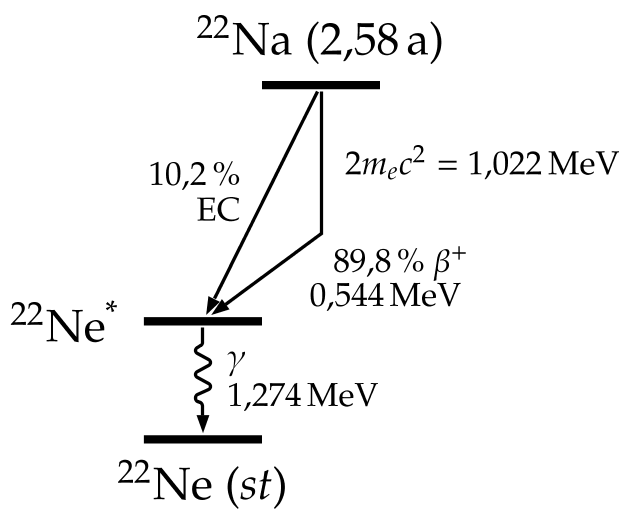
\includegraphics[width=1\textwidth]{Na22.png}
  \caption{Zerfallsschema von $^{22}$Na}
  \label{Na22}
\end{minipage}
\hfill
\begin{minipage}[t]{0.45\linewidth}  
     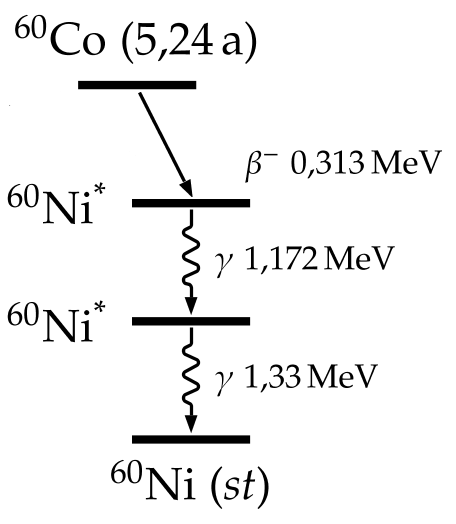
\includegraphics[width=0.7\textwidth]{Co60.png}
  \caption{Zerfallschema von $^{60}$Co}
  \label{Co60}
\end{minipage}
\end{figure}

\subsection{Koinzidenztheorie}
Eine Koinzidenz ist dann vorhanden, wenn zwei Detektoren
innerhalb eines Zeitintervalls, der Koinzidenzzeit, beide ein 
Signal messen. Unterschieden werden muss dabei zwischen den 
wahren Koinzidenzen und den zufälligen Koinzidenzen. Bei den wahren
Koinzidenzen können die beiden Signale einem einzigen physikalischen
Prozess zugeordnet werden. Die zufälligen Koinzidenzen entstehen
durch Detektion zweier Teilchen, die durch unabhängige physikalische
Vorgänge innerhalb der Koinzidenzzeit emittiert wurden. Im Experiment
soll erreicht werden, dass das Verhältnis von wahren zu zufälligen 
Koinzidenzen möglichst hoch ist, was durch geeignetes Wählen der 
Versuchsbedingungen erreicht wird.

Des Weiteren wird eine möglichst hohe Koinzidenzrate angestrebt. 
Die Einzelzählraten der beiden Detektoren ergeben sich aus
\begin{equation}
 Z_i=\varepsilon_i \omega_i Q, \;\;\; i=1,2,
\end{equation}
wobei $\varepsilon_i$ die Ansprechempfindlichkeit ist, $\omega_i$
der Raumwinkel, unter dem der Detektor die Signalqualle sieht und
$Q$ die Zerfallsrate der Probe. 

Um die Koinzidenzrate zu erhalten, muss die Zählrate des 1. Detektors
mit der Wahrscheinlichkeit multipliziert werden, dass der 2. 
Detektor ein Signal registriert. Diese Wahrscheinlichkeit kann 
vom Winkel abhängen, unter dem beide Signale gemessen werden, daher
wergibt sich für die Wahrscheinlichkeit einer Koinzidenz mit der 
Winkelverteilung $W(\vartheta)$:
\begin{equation}
 P(\vartheta)=\epsilon_2\omega_2 W(\vartheta)
\end{equation}
Die echte Koinzidenzrate ist daher:
\begin{equation}
 Z_{eK}=\varepsilon_1 \omega_1 \varepsilon_2 \omega_2 Q W(\vartheta)
\end{equation}

Um die Rate der zufälligen Koinzidenzen zu erhalten, betrachtet man die Wahrscheinlichkeit, dass
nach dem Messen von Detektor 1 innerhalb der Koinzidenzzeit $\tau$ ein unkorreliertes Signal im Detektor 2 
gemessen wird: $Z_2\cdot \tau$

Die Rate zufälliger Koinzidenzen ist daher:
\begin{equation}
 Z_{zK}=\tau Z_1Z_2
\end{equation}
Und das Verhältnis von echten zu zufälligen Koinzidenzen ist dann:
\begin{equation}
 \frac{Z_{eK}}{Z_{zK}}=\frac{1}{\tau Q}
\end{equation}
Für die Versuchsbedingungen bedeutet das, die Koinzidenzzeit so gering wie möglich zu wählen.
Außerdem sollten eine radioaktive Probe genutzt werden, deren Zerfallsrate nicht zu hoch ist,
aber dennoch nicht so gering,
dass man mit einem akzeptablen Zeitaufwand ein statistisch relevantes Ergebnis erhält.

\subsection{$\gamma$-$\gamma$-Winkelkorrelation}
Entstehen bei einem radioaktiven Zerfall oder einer Annihilation zwei Gamma-Quanten, sind sie
in ihrem Winkel zueinander korreliert. Das heißt, dass es eine Winkelverteilung der Intensität
der Koinzidenzen gibt, die charakteristisch für diese Art Zerfall ist. 

Der einfachste Fall ist die Annihilation von Positron und Elektron, bei der Gesamtimpuls von $~0$ 
erhalten bleibt. So werden die Gamma-Quanten unter einem Winkel von $180^\circ$ zueinander gemessen.

Im Fall eines Kerns, der über eine Kaskade von 2 Gamma-Quanten zerfällt wird die Annahme gemacht, dass
die Lebensdauer des Zwischenzustands so kurz ist, dass sich die Orientierung des Kerns im Vergleich 
zum ersten Zerfall nicht verändert. 

Allgemein kann die Winkelverteilung über die Formel
\begin{equation}
 W(\theta)=\sum_\nu A_\nu^{(1)} A_\nu^{(2)} P_\nu ( \cos \theta)
\end{equation}
angegeben werden. Dabei ind die $A_\nu^{(i)}$ Koeffizienten, die aus Tabellen abgelesen werden können.
$P_\nu(\cos \theta)$ sind Legendre-Polynome der $\nu$-ten Ordnung, wobei für nicht-polarisierte Strahlung
allerdings nur geradzahlige Polynome in der Winkelverteilung auftreten. Dadurch treten nur geradzahlige
Potenzen von $\cos \theta$ auf, was die Winkelverteilung $W(\theta)$ zu einer zu $90^\circ$ symmetrischen
Funktion macht. Es reicht daher die Messung auf einen Bereich von $\theta=0^\circ$ bis $90^\circ$ zu 
beschränken.

\section{Versuchsaufbau und Messgeräte}

Zum Nachweise der $\gamma$-Strahlung werden in diesem Versuch zwei NaI-Szintillationszähler verwenden. Dieser besteht prinzipiell aus einem Szintillator und einem Photomultiplier und ist schematisch in Abbildung \ref{PMT} dargestellt. Treffen energiereiche Photonen auf den Szintillationskristall, so werden durch die oben beschriebenen Wechselwirkungsprozesse Elektronen ausgelöst. Diese können Atome im Kristall anregen oder ionisieren, wodurch Fluoreszenzphotonen emittiert werden. Die vom Szintillator emittierten Photonen werden über einen Lichtwellenleiter an einen Photomultipliert weitergeleitet und schlagen in diesem über den Photoeffekt Elektronen aus den Atomen, welche kaskadenartig über eine zwischen einer Vielzahl an Dynoden angelegten Spannung vervielfacht und in ein messbares Signal umgewandelt werden. Als Szintillationskristall dient in unserem Fall ein mit Thallium dotierter Natriumiodid-Kristall. Die Thalliumatome dienen als Leuchtzentren im Szintillator. Ihre Anregungsenergie liegt innerhalb der Bandlücke des Natriumiodids, wodurch sie leichter angeregt werden können, was wiederum in einer guten Photonenausbeute im sichtbaren Bereich resultiert. Die Größe des Kristalls wird bei Szintillatoren so gewählt, dass die Wahrscheinlichkeit für die genannten Wechselwirkungsprozesse ausreichend groß ist. 

\begin{figure}[htbp]  
     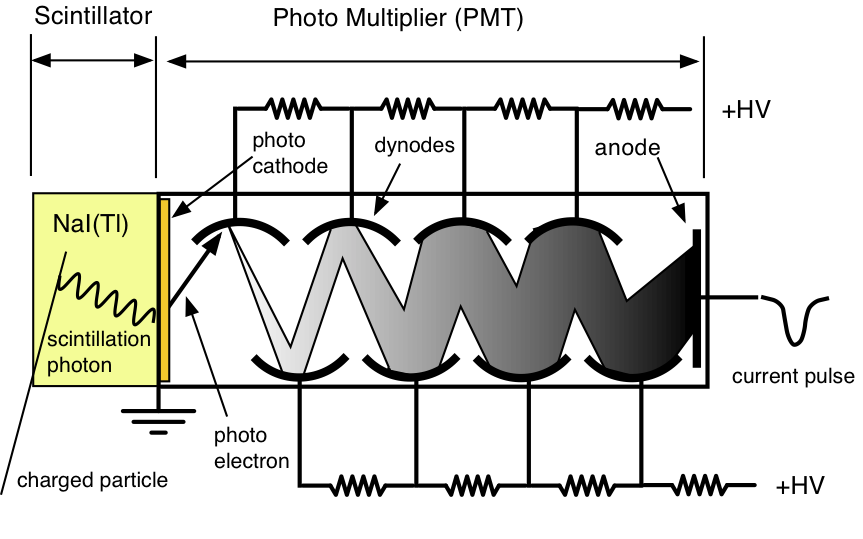
\includegraphics[width=0.7\textwidth]{PMT.png}
  \caption{Schematischer Aufbau eines NaI-Szintillationszählers}
  \label{PMT}
\end{figure}


\section{Versuchsteil 1}


\subsection{Durchführung}


\subsection{Auswertung}


\section{Versuchsteil 2}



\subsection{Durchführung}



\subsection{Auswertung}




\section{Zusammenfassung/Fazit}

Text


\end{document}